% 球体的万有引力

\subsection{均匀圆环的引力场}
我们先来看一个跟简单的问题. 如\autoref{SphF_fig1}, 求一个质量为 $M$ 半径为 $R$ 的圆环对圆环轴线上任意一点产生的引力场 $P$ 产生的引力场, 已知点 $P$ 到圆环上任意一点的连线长度为 $r$, 与 $z$ 轴的夹角为 $\theta$.

\begin{figure}[ht]
\centering
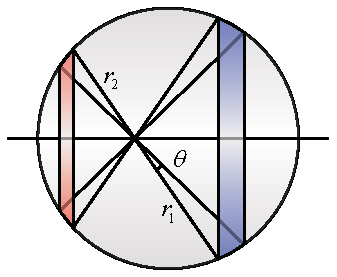
\includegraphics[width=5.2cm]{./figures/SphF1.pdf}
\caption{圆环的引力场} \label{SphF_fig1}
\end{figure}

由问题的对称性, 所求引力场由 $P$ 指向 $O$. 若我们将圆环划分为许多小段, 每小段质量为 $m_i$, 则 $m_i$ 在点 $P$ 产生的引力场在 $PO$ 方向的分量为
\begin{equation}
g_i = \frac{Gm_i}{r^2}\cos\theta
\end{equation}
所以总引力场大小等于
\begin{equation}\label{SphF_eq2}
g = \sum_i g_i = \frac{GM}{r^2}\cos\theta
\end{equation}

\subsection{均匀球壳的引力场}

\begin{figure}[ht]
\centering
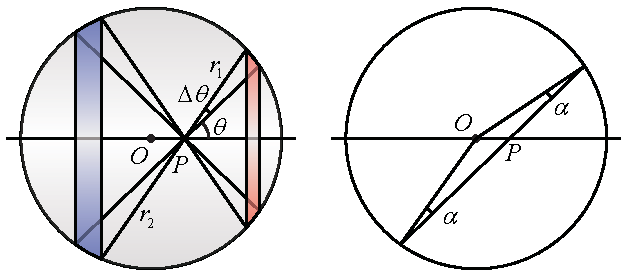
\includegraphics[width=10cm]{./figures/SphF2.pdf}
\caption{几何法证明} \label{SphF_fig2}
\end{figure}

我们现在来证明一个质量面密度为 $\sigma$ 的均匀球壳在其内部一点 $P$ 产生的引力场为零. 如\autoref{SphF_fig2}, 令球心为 $O$, 并过 $OP$ 作一个轴, 这样球面上任意一点都对应一个张角 $\theta$. 根据不同的 $\theta$ ($0 < \theta < \pi/2$)可将球壳划分为许多对细圆环, 每个圆环对应一个 $\Delta\theta$. 当 $\Delta\theta\to 0$ 时, 如果能能明任意一对细圆环在 $P$ 点产生的引力场都能互相抵消, 那么球壳对 $P$ 点的总引力场就为零.

我们先要求出两个圆环的面积, 以左图中右边的圆环为例, 圆环的周长为 $2\pi r_1\sin\theta$, 当 $\Delta\theta\to 0$ 时, 圆环的宽度为 $r_1\Delta\theta/\cos\alpha$ ($\alpha$ 的定义见右图), 所以圆环的面积等于周长乘以宽度, 再乘以面密度 $\sigma$ 得到右圆环的质量
\begin{equation}
M_1 = 2\pi r_1^2 \sigma \Delta\theta\sin\theta /\cos\alpha
\end{equation}
同理, 左圆环的质量为
\begin{equation}
M_2 = 2\pi r_2^2 \sigma \Delta\theta\sin\theta /\cos\alpha
\end{equation}
将 $M_1, r_1$ 和 $M_2, r_2$ 分别代入\autoref{SphF_eq2} 可得 $g_1 = g_2$ 即两圆环在 $P$ 点产生的引力场大小相等, 方向相反, 总引力场为零. 证毕.